\section{Information Theory} \label{sec:information-theory}
The birth of the field of \textit{information theory} is usually traced back to the seminal paper \enquote{A Mathematical Theory of Communication} \citep{Shannon1949} where the mathematical basis for the quantification of the amount of \textit{information} transmissible over a noisy channel was set. 
In his words, \enquote{the fundamental problem of communication is that of reproducing at one point, either exactly or approximately, a message selected at another point}.
The concepts of field are broad enough to have influenced practically every other scientific discipline and deep enough to have made the \enquote{digital age} possible, for example by enabling the creation of ever more complicated coding schemes for the compression, reconstruction and obfuscation of digital data.

\subsection{Entropy} \label{subsec:entropy}
In classical mechanical statistics, \textit{entropy} can be seen as a measure of the uncertainty, or randomness, of a physical system.  
This concept was reapplied by Shannon to measure the amount of randomness, the converse of information, in a random variable.
\begin{definition}[Entropy] \label{def:entropy}
	The entropy $\Eta(X)$ is defined as the expected amount of information content carried by random variable $X$ \citep{Schneider2005}:
\begin{equation*}
	\Eta(X) = -\sum\limits_{x \in \mathcal{X}} \mathbb{P}(X=x) \log_{b} \mathbb{P}(X=x) \,.
\end{equation*}
\end{definition}
The base $b$ of the logarithm defines the unit of measure.  
Shannon used $b=2$ as he was dealing with the transmission of digital, binary-coded data; in this case the unit of measure would be \textit{bits}.

The entropy of a generic random variable's probability mass function is a \textit{unimodal functional} (a function whose codomain is in the space of functions is called a functional) whose domain is the subset $[0,1]$.
Its maximum $1$ is reached when applied to a uniform probability mass function while its minima appear in the presence of \textit{degenerate probability mass distributions} i.e., those that are localised at a single value (all values have probability zero, except one that is certain).

As always, we can define a \textit{conditional version} of the notion:
\begin{definition}[Conditional Entropy] \label{def:conditional-entropy}
	The conditional entropy $\Eta(Y \mid X)$ is defined as:
\begin{equation*}
	\Eta(Y | X)=-\sum_{x \in \mathcal{X}, y \in \mathcal{Y}} \mathbb{P}(X=x,Y=y) \log_{b} \frac{\mathbb{P}(X=x,Y=y)}{\mathbb{P}(X=x)} \,.
\end{equation*}
\end{definition}

The simplest example of how information entropy characterises a random variable $X$, is in imagining $X$ as modelling a coin and being tasked with predicting the probability of the outcome of a throw being \textit{heads}.
If the coin is fair, we will not be any more \enquote{surprised} to see that the outcome is heads instead of tails; the entropy is maximum, as there is maximum uncertainty regarding the outcome.
However, if the coin is not fair and tails is more probable than heads, then we will be more surprised if we see that the outcome is heads.  
The entropy is sub-maximal because there is less uncertainty regarding the outcome due to the fact that tails is more probable than heads.
If one of the outcomes is impossible, for example if the coin has two heads, then the entropy of the coin is $0$, as there is no uncertainty regarding the result of a toss.
All these cases can easily be understood by looking at Figure \ref{fig:entropy-plot}.

%\begin{tikzpicture}[declare function = {b(\k, \n, \p) = \n!/(\k!*(\n-\k)!)*\p**\k*(1-\p)**(\n-\k);}]
%\begin{axis}[domain=0:10,
%  samples=100,
%  enlarge x limits=false,
%  grid=both,
%  no markers,
%  axis equal
%  ]
%\addplot +[thick] {sum [k=0:\N] -b(k,\N,x)*log(b(k,\N,x))/log(2)};
%\end{axis}
%\end{tikzpicture}

\todo[inline]{generare io figura}

\begin{figure}[htbp]
\centerline{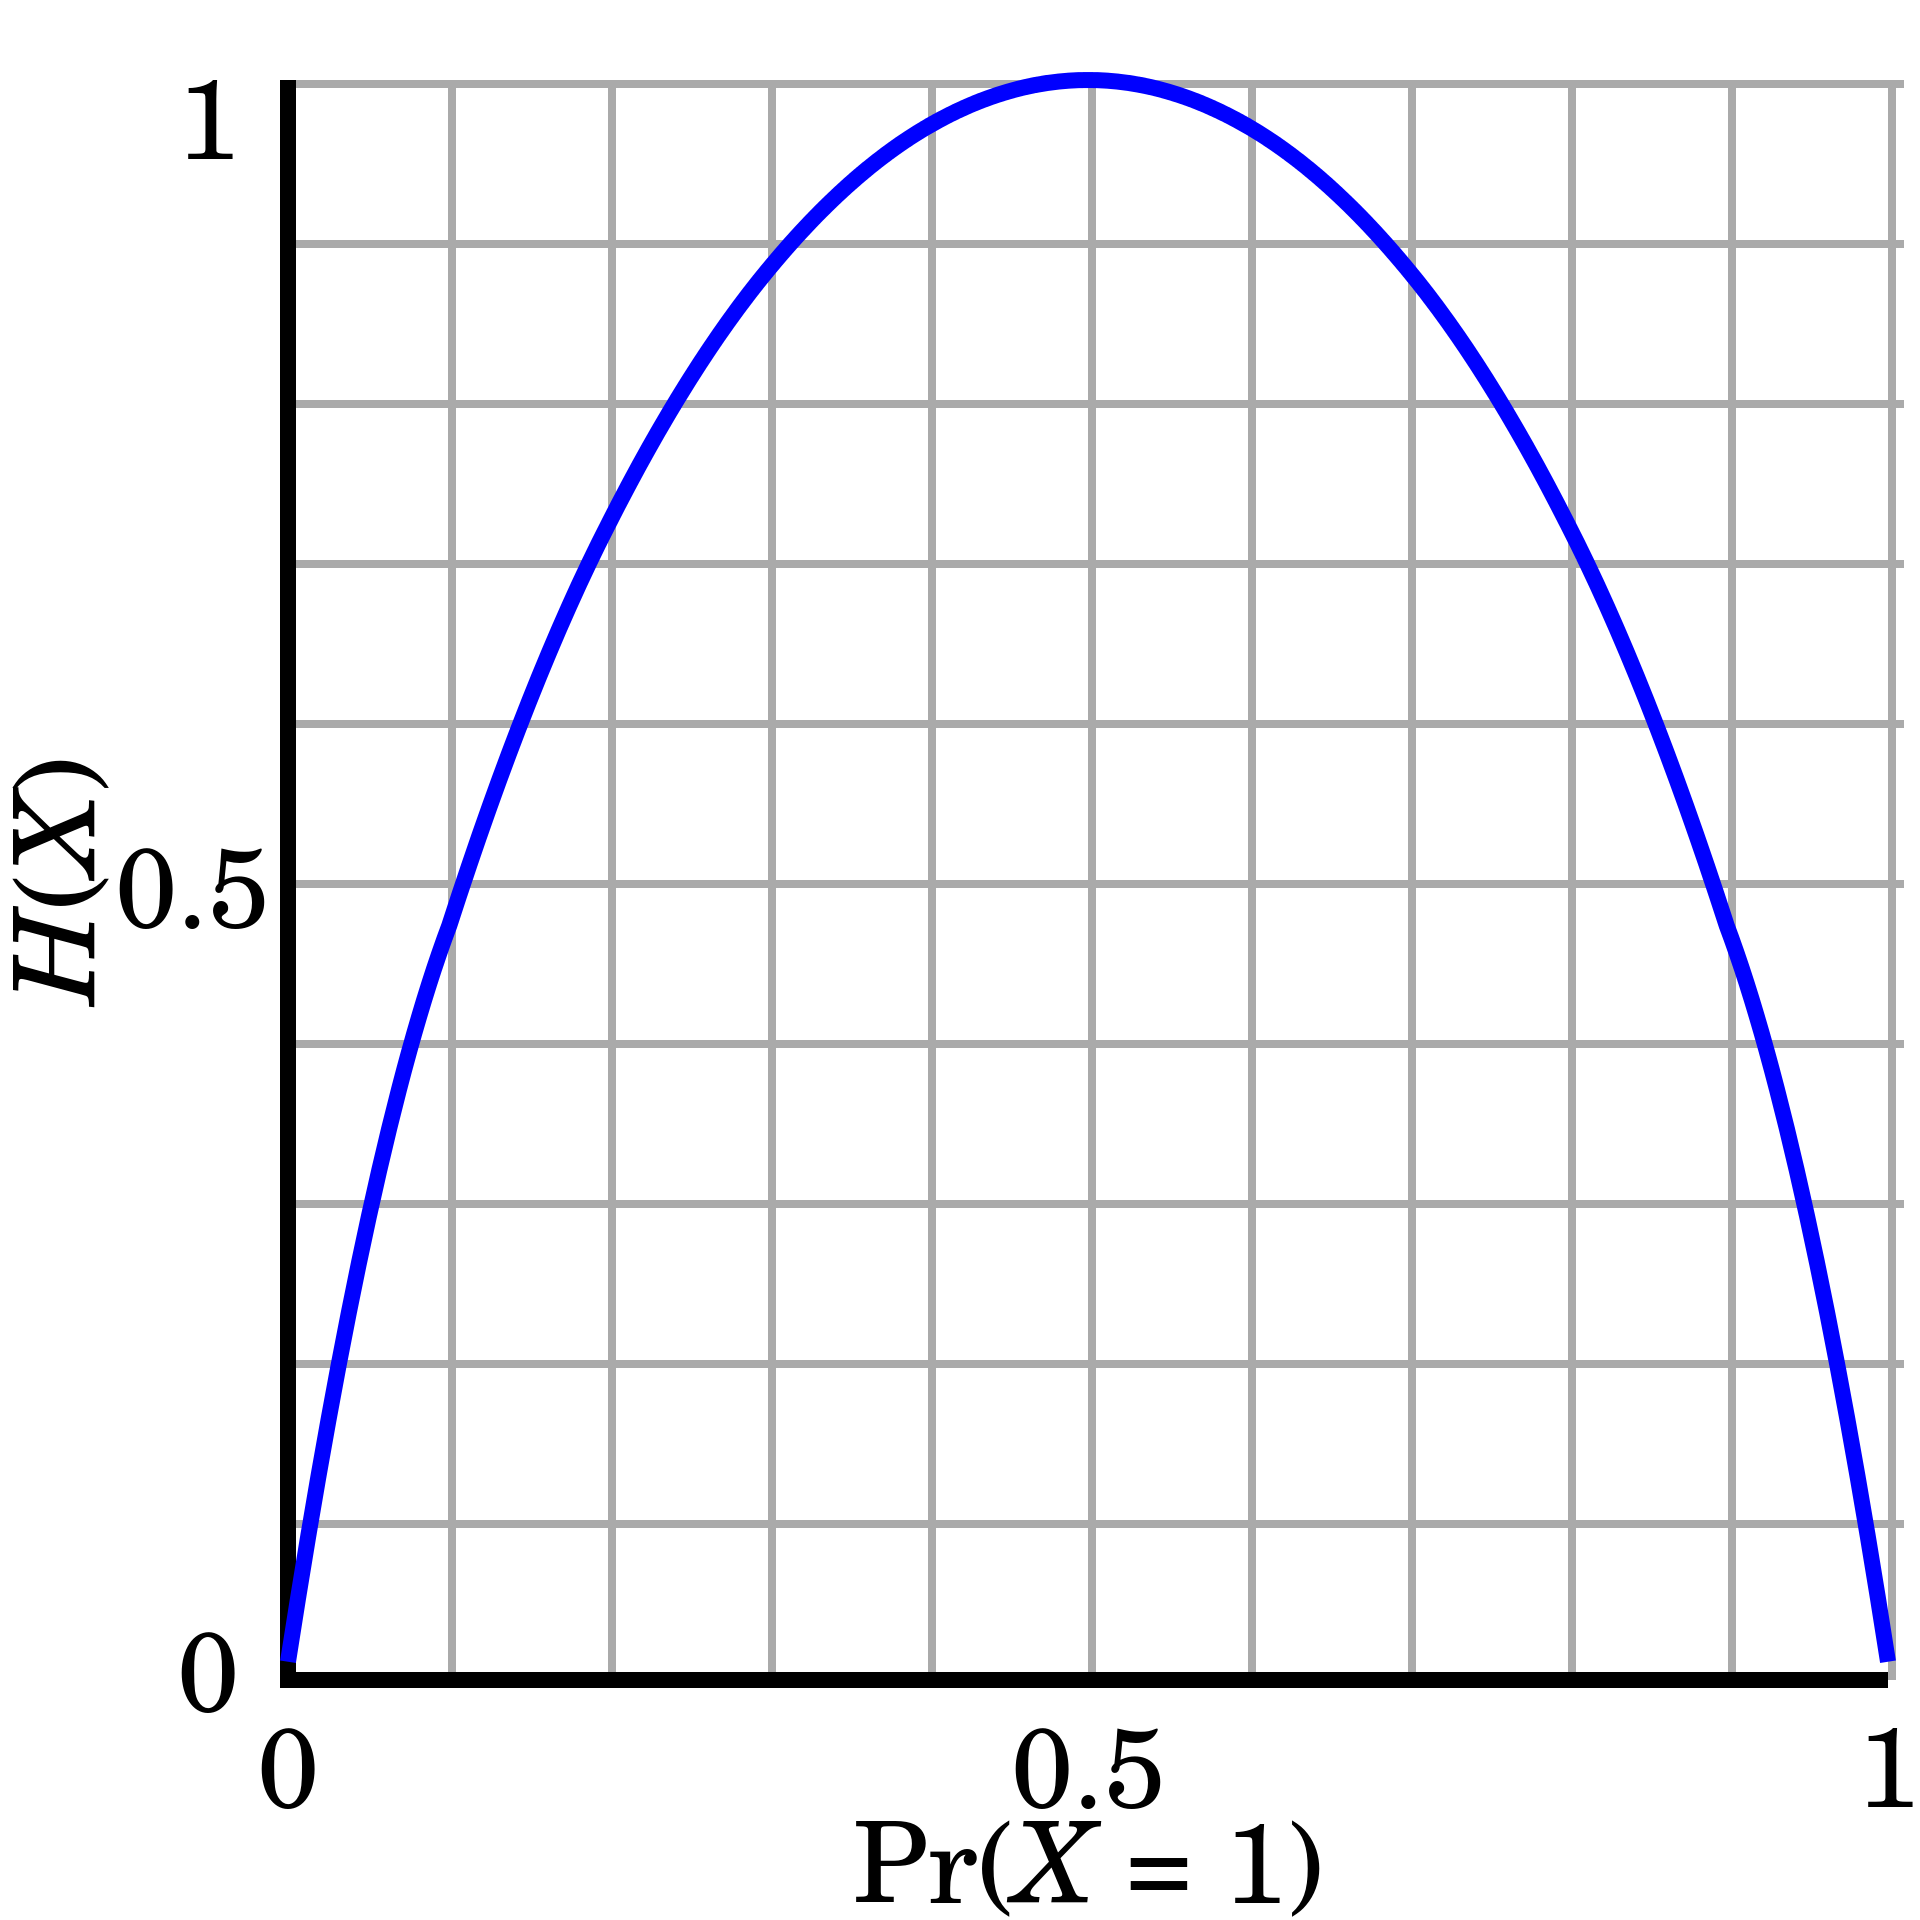
\includegraphics[width=0.5\textwidth]{mathematical-background/images/entropy-plot}}
\caption{Entropy of a fair coin with the outcome $X=1$ of the random variable representing heads [original work by Brona, published on Commons at Image:Binary entropy plot.png. Converted to SVG by Alessio Damato, CC BY-SA 3.0, https://commons.wikimedia.org/w/index.php?curid=1984868]}
\label{fig:entropy-plot}
\end{figure}

Plain entropy might be not the appropriate tool when trying to characterise random variables with codomains of different cardinality.
Let us suppose that the objective is to find the variable with the least \enquote{entropic} distribution and imagine that their values have all been generated by the same process, say Gaussian.
Simply calculating their entropies and ordering them according to this criterion will bias the selection process towards the variables with smallest cardinality.
This is because we supposed them to be homoscedastic so there will naturally be less uncertainty when there are fewer possible outcomes.
This can easily be understood by imagining the distributions to all be random uniform
(this topic is further analysed in Subsection \ref{subsec:entropy-based-selection}).

To obviate to this problem we need to \textit{normalise} the entropy so that different-sized variables can be directly compared to each other.
To achieve this, we can look at a measure of \textit{normalised entropy}.
\begin{definition}[Normalised Entropy] \label{def:normalisedentropy}
The normalised entropy - or efficiency - or random variable $X$ with domain $\mathcal{X}$ is given by:
	\begin{equation*} 
 	\Eta(X)=-\sum\limits_{x \in \mathcal{X}} \frac{\mathbb{P}(X=x) \log _{b}\mathbb{P}(X=x)}{\log_{b}(n)} \,.
\end{equation*}
\end{definition}
From Definition \ref{def:normalisedentropy} it can be seen that $\Eta(X) \in [0,1]$; it is thus a normalised measure that is comparable across different-sized variables.
This ratio expresses the amount of entropy found in the distribution compared to the maximum possible entropy when using $n$ symbols, the case corresponding to the uniform distribution:
\begin{equation}
\mathrm{H}\left(\underbrace{\frac{1}{n}, \ldots, \frac{1}{n}}_{n}\right) = - \sum\limits_{i=1}^n \frac{1}{n} \log _{b} \left( \frac{1}{n} \right) = -n \cdot \frac{1}{n} \log _{b} \left( \frac{1}{n} \right) = - \log _{b} \left( \frac{1}{n} \right) = \log _{b}(n) 
\end{equation}   

\subsection{Mutual Information} \label{subsec:mutual-information}
Another way of characterising the interrelatedness of two variables is through the concept of \textit{mutual information}, as defined in \citet{Cover2006}, that is closely linked to entropy (Definition \ref{def:entropy}).
\begin{definition}[Mutual Information]
	The mutual information of two random variables $X$ and $Y$ with domains $\mathcal{X}$ and $\mathcal{Y}$ is given by:
	\begin{equation*} \label{def:mutual-information}
		I(X,Y) = \sum\limits_{x \in \mathcal{X}} \sum\limits_{y \in \mathcal{Y}} \mathbb{P}(X=x,Y=y) \log_{b} \left( \frac{\mathbb{P}(X=x,Y=y)}{\mathbb{P}(X=x) \mathbb{P}(Y=y)} \right) \,.
	\end{equation*}
\end{definition}
NB: In Information Theory, the convention is that $0 \log(0) = 0$.

$I(X,Y)$, intuitively, measures the amount of information that $X$ and $Y$ share and can also be seen as the degree to which one variable is informative of the other.
If $X$ and $Y$ are independent then they share no mutual information and something about one of the two gives no information about the other.
This can be immediately understood by rewriting Definition \ref{def:mutual-information} as:
\begin{equation}
	I(X,Y) = H(X) - H(X|Y) = H(Y) - H(Y|X)
\end{equation}
The mutual information I(X,Y) is the reduction in uncertainty of one of the variables given the knowledge of the other.
If $X$ and $Y$ are perfectly correlated (correlation $\rho(X,Y)$, as defined by \citet{Stolp2006}, is a measure of the degree to which two random variables are linearly dependent, perfect correlation means $\rho(X,Y)= \pm 1$) then they both convey the same amount of information and $I(X,Y)$ is equal to the entropy i.e., $\Eta(X) = \Eta(Y)$.

\subsection{Kullback-Leibler Divergence} \label{subsec:kl-divergence}
The \textit{Kullback-Leibler divergence} was first defined by \citet{Kingman2007} and is another measure for the difference between two random variables, that is also closely related to the concepts of entropy (Subsection \ref{subsec:entropy}) and of mutual information (Subsection \ref{subsec:mutual-information}).
\begin{definition}[Kullback-Leibler Divergence] \label{def:kl-divergence}
	The Kullback-Leibler divergence $D_{KL}(Y \parallel X)$ - also known as information gain - between two random variables $Y$ and $X$, whose distribution is defined on the same probability space, is given by:
	\begin{equation*} 
		D_{KL}(Y \parallel X)=-\sum\limits_{x \in \mathcal{X}} \mathbb{P}(Y=y) \log_{b} \left(\frac{\mathbb{P}(X=x)}{\mathbb{P}(Y=y)}\right) = \sum\limits_{x \in \mathcal{X}} \mathbb{P}(Y=y) \log_{b} \left(\frac{\mathbb{P}(Y=y)}{\mathbb{P}(X=x)}\right) \,.
	\end{equation*}
\end{definition}
As always, the base $b$ of the logarithm defines the unit of measure; KL divergence is defined for any $b$.

Intuitively, it can be seen as measuring the amount of information gained when revising one's beliefs from the distribution of $X$ to the distribution of $Y$.
Unlike information gain, it is not a \textit{distance measure} as it is evidently asymmetric i.e., $D_{\mathrm{KL}}(Y \parallel X) \neq D_{\mathrm{KL}}(X \parallel Y)$; if there is an \textit{information gain} when moving from $X$ to $Y$, there is an \textit{information loss} when revising one's beliefs from $Y$ to $X$.

The \textit{mutual information} $I(X,Y)$ is related to the \textit{information gain} by:
\begin{equation} \label{def:mutual-information-kl-divergence-equivalence}
	I(X,Y) = D_{\mathrm{KL}}(\mathbb{P}(X,Y) \| \mathbb{P}(X=x) \mathbb{P}(Y) )
\end{equation}
That is, the mutual information of two random variables is equal to the difference in information content between the product of the marginals and the joint distribution.
This can better be understood through the terms of information theory: the mutual information of $X$ and $Y$ is the extra number of symbols needed to discriminate between the distributions of $X$ and $Y$, when they are coded using their marginal distributions and not their joint.
This is to be expected because the definition of mutual information is exactly the information shared by $X$ and $Y$ and all that is needed to discriminate between the marginals is this particular \enquote{set} of information.
The equivalence shown in Equation \ref{def:mutual-information-kl-divergence-equivalence} can be proved by simply substituting $X=\mathbb{P}(X=x) \mathbb{P}(Y)$ and $Y=\mathbb{P}(X,Y)$ into Definition \ref{def:kl-divergence}; the result will be Definition \ref{def:mutual-information}.

\subsection{Hamming Distance} \label{subsec:hamming-distance}
The \textit{Hamming Distance} is a widely-used distance measure that quantifies the similarity of strings.
\begin{definition}[Hamming Distance] \label{def:hamming}
	The Hamming Distance $D_H(x,y)$ between two vectors $x$ and $y$ is given by:
	\begin{equation}
		d_H(x,y) = \sum\limits_i \Gamma(x_i, y_i) \,,
	\end{equation}
	with $\Gamma(i,j)$ defined as:
	\begin{equation}
		\Gamma(i,j) = 
		\begin{cases}
			0 \quad i \neq j \\
			1 \quad i = j	
		\end{cases} \,.
	\end{equation}
\end{definition}
Given strings of characters, or more in general vectors over some field, of equal length, their Hamming Distance is the number of positions where they differ.
It can be seen as the number of substitutions needed to transform one into the other.

This is a valid distance measure because:
\begin{itemize}
  \item it is non-negative: $D_H(x,y) \geq 0$
  \item it fulfils the identity of indiscernibles: if $x = y$ then $D_H(x,y)=0$
  \item it respects the \textit{Triangle Inequality}: $D_H(x,y) \leq D_h(x,z) + D_H(z,y) $
\end{itemize}

As an example, strings $x=01234$ and $y=15244$ have $D_H(x,y)=2$, as they differ in two positions.

\subsection{Jaccard Distance} \label{subsec:jaccard-distance}
The \textit{Jaccard Distance} is a popular metric to measure the similarity of sets.
\begin{definition}[Jaccard Similarity Coefficient] \label{def:jaccard}
	The Jaccard Similarity Coefficient $J(A,B)$ of two sets $A$ and $B$ is given by:
	\begin{equation*}
		J(A,B) = \frac{|A \cap B |}{| A \cup B |} \,.
	\end{equation*}
\end{definition}
\begin{definition}[Jaccard Distance]
	The Jaccard Distance $D_J(A,B)$ between two sets $A$ and $B$ is given by:
	\begin{equation*}
		D_J(A,B) = 1 - J(A,B) \,.
	\end{equation*}
\end{definition}

This is a valid distance measure because:
\begin{itemize}
  \item it is non-negative: $D_J(A,B) \geq 0 \quad \forall A, B$
  \item it fulfils the identity of indiscernibles: if $A = B$ then $D_J(A,B)=0$
  \item it respects the \textit{Triangle Inequality}: $D_J(A,B) \leq D_J(A,C) + D_J(C,B) $
\end{itemize}

For example, the sets $A = \{ 0, 2, 3, 4, 1 \}$ and $B = \{ 1, 3, 5 \}$ have $D_J(A,B) = \frac{2}{6}$, as their intersection is of cardinality 2 and their union of cardinality 6.
